\section{\textcolor{red}{Experiments}}
\label{5.0}
\subsection{Experimental Setup}
\medskip
\noindent
\textit{Datasets and Pre-trained Models:} We evaluate BID-LoRA on classification and face recognition tasks. For classification, we use CIFAR-100 \cite{krizhevsky2009learning} and adopt data-efficient image transformers \cite{touvron2021training} as the backbone. For face recognition, we use \textcolor{red}{VGGFace2~\cite{cao2018vggface2}, sampling 200 identities}, with a Face Transformer \cite{zhong2021face} as the backbone. We use $D_r$ as 10\% of $D^\text{full}_r$ as buffer. We use uniform rank 8 for both retain and new adapters, while the forget adapter uses rank 4. \textcolor{red}{All BID-LoRA results are averaged over 3 random seeds and reported as mean$_{\pm\text{std}}$.}

\medskip
\noindent
\textit{Evaluation Protocol:} We implement a six-task evaluation protocol where the model progressively transitions from classes 0-29 to 60-89. Each task involves: (i) retaining 20 classes, (ii) forgetting 10 classes, and (iii) learning 10 new classes. Starting from a pre-trained checkpoint on classes 0-29, each subsequent task slides the class window by 10 positions: task 1 operates on classes 10-39, task 2 on classes 20-49, continuing until task 6 operates on classes 60-89 (Fig.~\ref{fig:sliding_window}). This sliding window design validates true continual adaptation through simultaneous learning and forgetting. Our protocol offers key advantages over existing methods. First, it tests longevity and sustainability claims often questionable under extended evaluation. Second, over the complete cycle, every piece of pretrained knowledge is systematically replaced, providing comprehensive assessment of adaptability. Third, this extensive protocol proves our approach's genuineness through sustained performance across multiple knowledge transitions rather than cherry-picked scenarios.

\medskip
\noindent
\textit{Theoretical Best:} We compare all baseline methods and our approach against Oracle-model performance, which serves as the theoretical and practical upper bound. Oracle models are obtained by directly training on each target class range, such as classes 10-39 for task 1 and classes 20-49 for task 2, continuing through task 6, without any low-rank adaptations, incremental learning, or unlearning approaches. This provides a clean baseline that follows the same 6-task sliding window protocol, allowing us to measure how close our continual adaptation approach comes to optimal performance. The Oracle comparison quantifies how close our continual adaptation approach comes to optimal retraining performance.

\medskip
\noindent
\textit{Metrics:} 
We evaluate our approach based on the performance of forgotten, retained, and newly learned classes using class accuracy, Membership Inference Attack (MIA) success rate, and KL divergence. Following Huang et al.~\cite{huang2025unified}, we define: forget accuracy $Acc_f$ as \textcolor{red}{cumulative} performance on \textcolor{red}{all previously} forgotten data\textcolor{red}{, measuring forgetting persistence}, retain accuracy $Acc_r$ as performance on retained data, new accuracy $Acc_{n}$ as performance on newly added data, and overall accuracy $Acc_o$ as performance across combined retained and new classes. To verify effective unlearning, we measure the MIA success rate as suggested by~\cite{choquette2021label}, and compute KL divergence between each model and the oracle model to assess logit-level similarity. We also report the tunable ratio, defined as the proportion of parameters updated during CLU steps, to indicate practical usability under resource-constrained scenarios.


\begin{figure}[!htbp]
    \centering
    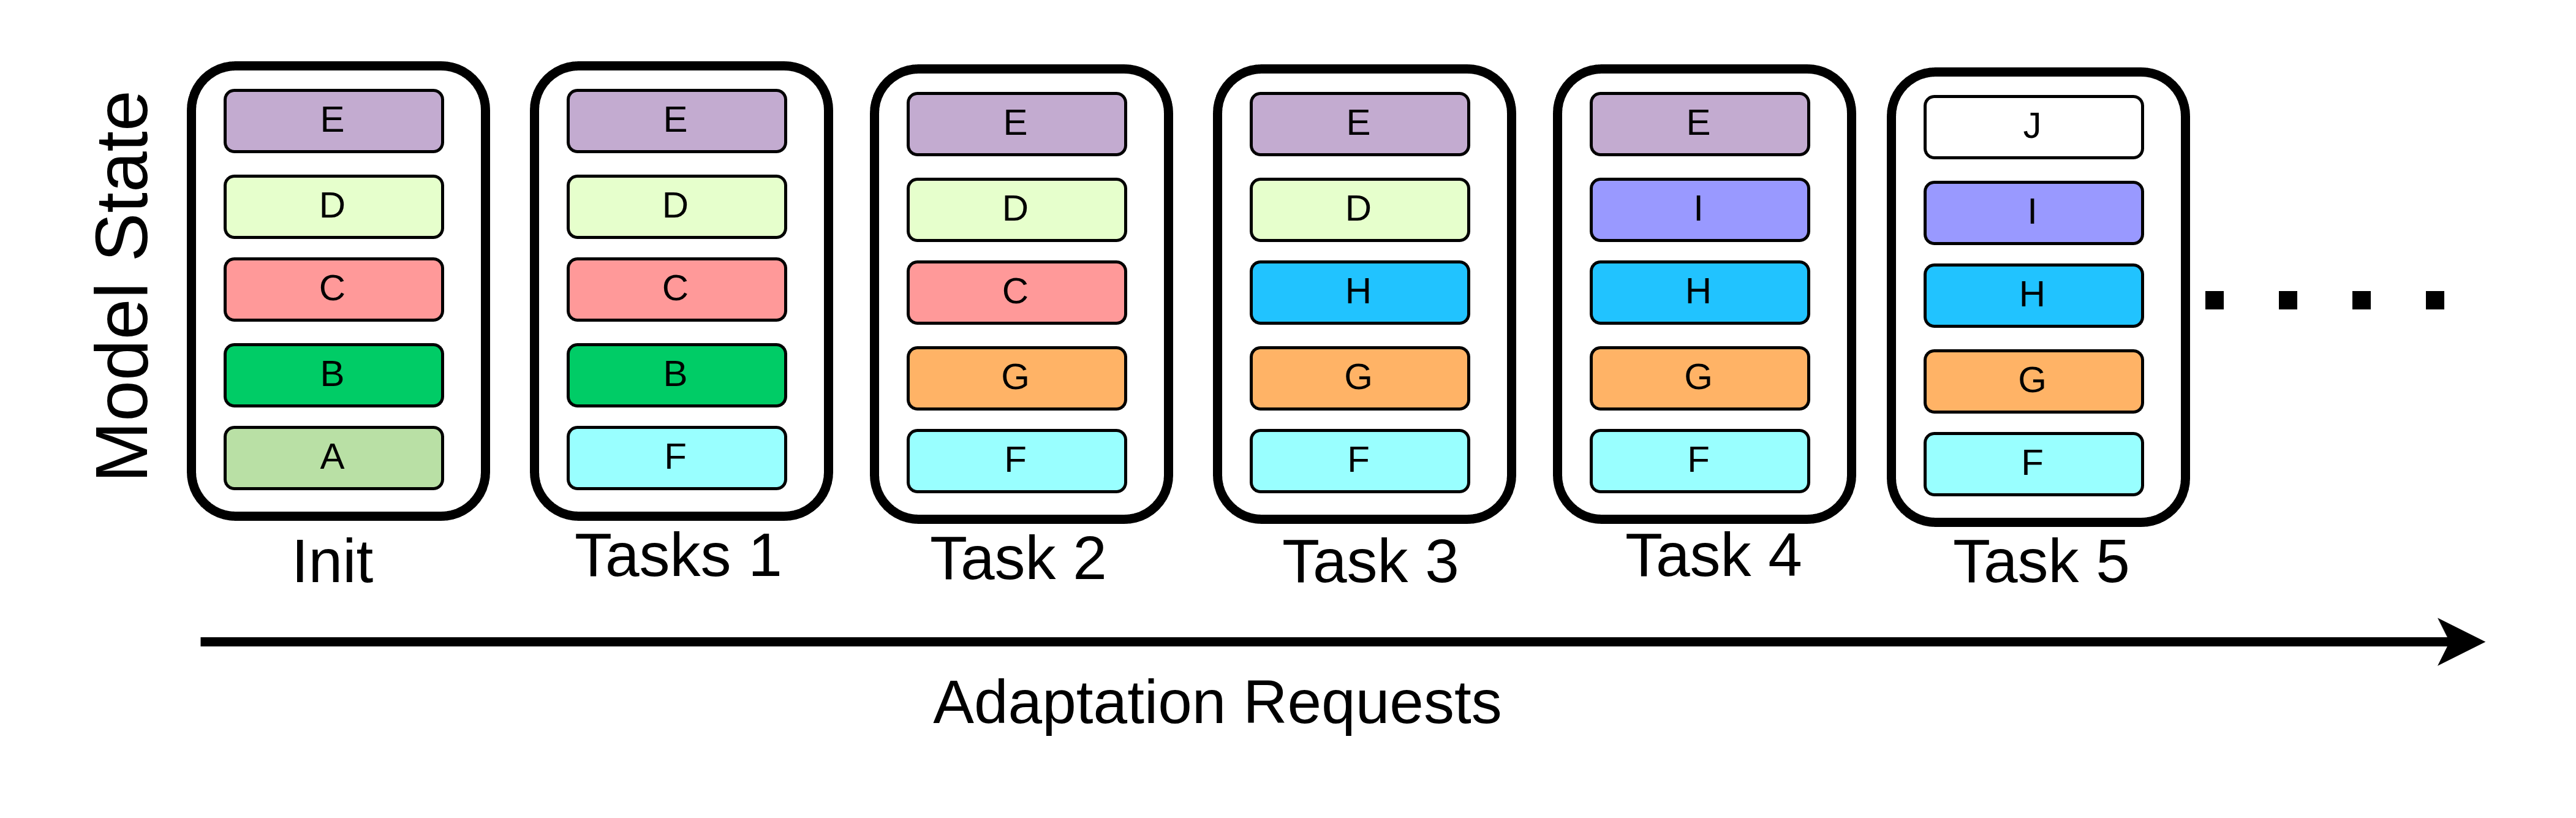
\includegraphics[width=0.75\textwidth]{images/steps.png}
    \caption{Illustration of continual adapting evaluation protocol.}
    \label{fig:sliding_window}
\end{figure}


Ideally, $Acc_f$ should approach zero, while $Acc_r$, $Acc_{n}$, and $Acc_o$ should align with the oracle model's performance. The tunable ratio should approach zero for parameter efficiency. The MIA success rate should approximate 0.5, indicating the adversary cannot distinguish between unlearned and never-seen knowledge. KL divergence should approach zero, indicating no difference at the logit level between the oracle and adapted models.
\subsection{Baseline Implementations}
\label{5.4}

\medskip
\noindent
For baselines, we adopt implementations of existing CLU methods discussed in Section~\ref{2.4}. These include LSF by Shibata et al.~\cite{shibata2021learning}, which introduced the CLU problem and provided an initial solution. We also compare against CLPU-DER++ by Liu et al.~\cite{liu2022continual}, which employs temporal networks for cleaner removal of forget knowledge, UniCLUN by Chatterjee et al.~\cite{chatterjee2024unified}, a student-teacher distillation approach, UnCLe by Adhikari et al.~\cite{adhikari2025unlearning}, which explores hypernetworks for data-free unlearning, and UG-CLU by Huang et al.~\cite{huang2025unified}, a weight saliency-based method.

\subsection{Results Discussion}
\label{5.5}

\medskip
\noindent
Tables~\ref{tab:classification} and~\ref{tab:face_recognition} present results for CIFAR-100 classification and \textcolor{red}{VGGFace2} recognition. BID-LoRA achieves first (\textcolor{green}{green}) or second-best (yellow) performance across nearly all metrics while using only $\approx$ 5.08\% tunable parameters compared to 100\% for all baselines.

\medskip
\noindent
\textit{Unlearning Analysis:} BID-LoRA maintains forget accuracy between 0--0.93\% on CIFAR-100, with 0.93\% in Task 1, 0.27\% in Task 2, and 0.13\% in Task 3, and 0--0.88\% on face recognition, confirming effective unlearning. On CIFAR-100, BID-LoRA achieves the best or second-best overall accuracy in \textcolor{red}{3 of 6} tasks: 76.03\% (Task 1), 76.71\% (Task 4), and 73.51\% (Task 6). \textcolor{red}{MIA and KL divergence results are reported in the ablation study (Section~\ref{7.0}). This parameter efficiency comes with a modest accuracy trade-off: baselines updating 100\% of parameters occasionally match or exceed BID-LoRA's overall accuracy on individual tasks, though at roughly 20\texttimes\ the tunable-parameter cost.}

\medskip
\noindent
\textit{Knowledge Leakage Analysis:} Knowledge leakage, measured by overall accuracy degradation across tasks, remains minimal for BID-LoRA. While baseline methods such as LSF~\cite{shibata2021learning} and UniCLUN~\cite{chatterjee2024unified} show cumulative accuracy drops of 3--8\% from Task 1 to Task 6, BID-LoRA maintains stable performance with only 2.52\% variation on CIFAR-100 (76.03\% $\rightarrow$ 73.51\%) and \textcolor{red}{5.86\% variation on face recognition, ranging from 87.03\% to 92.89\% across Tasks 1--12, demonstrating minimal knowledge leakage despite twice as many adaptation cycles on the larger benchmark. KL divergence results are reported in the ablation study (Section~\ref{7.0}).}

\begin{figure}[!htbp]
    \centering
    \begin{subfigure}[b]{0.38\linewidth}
        \centering
        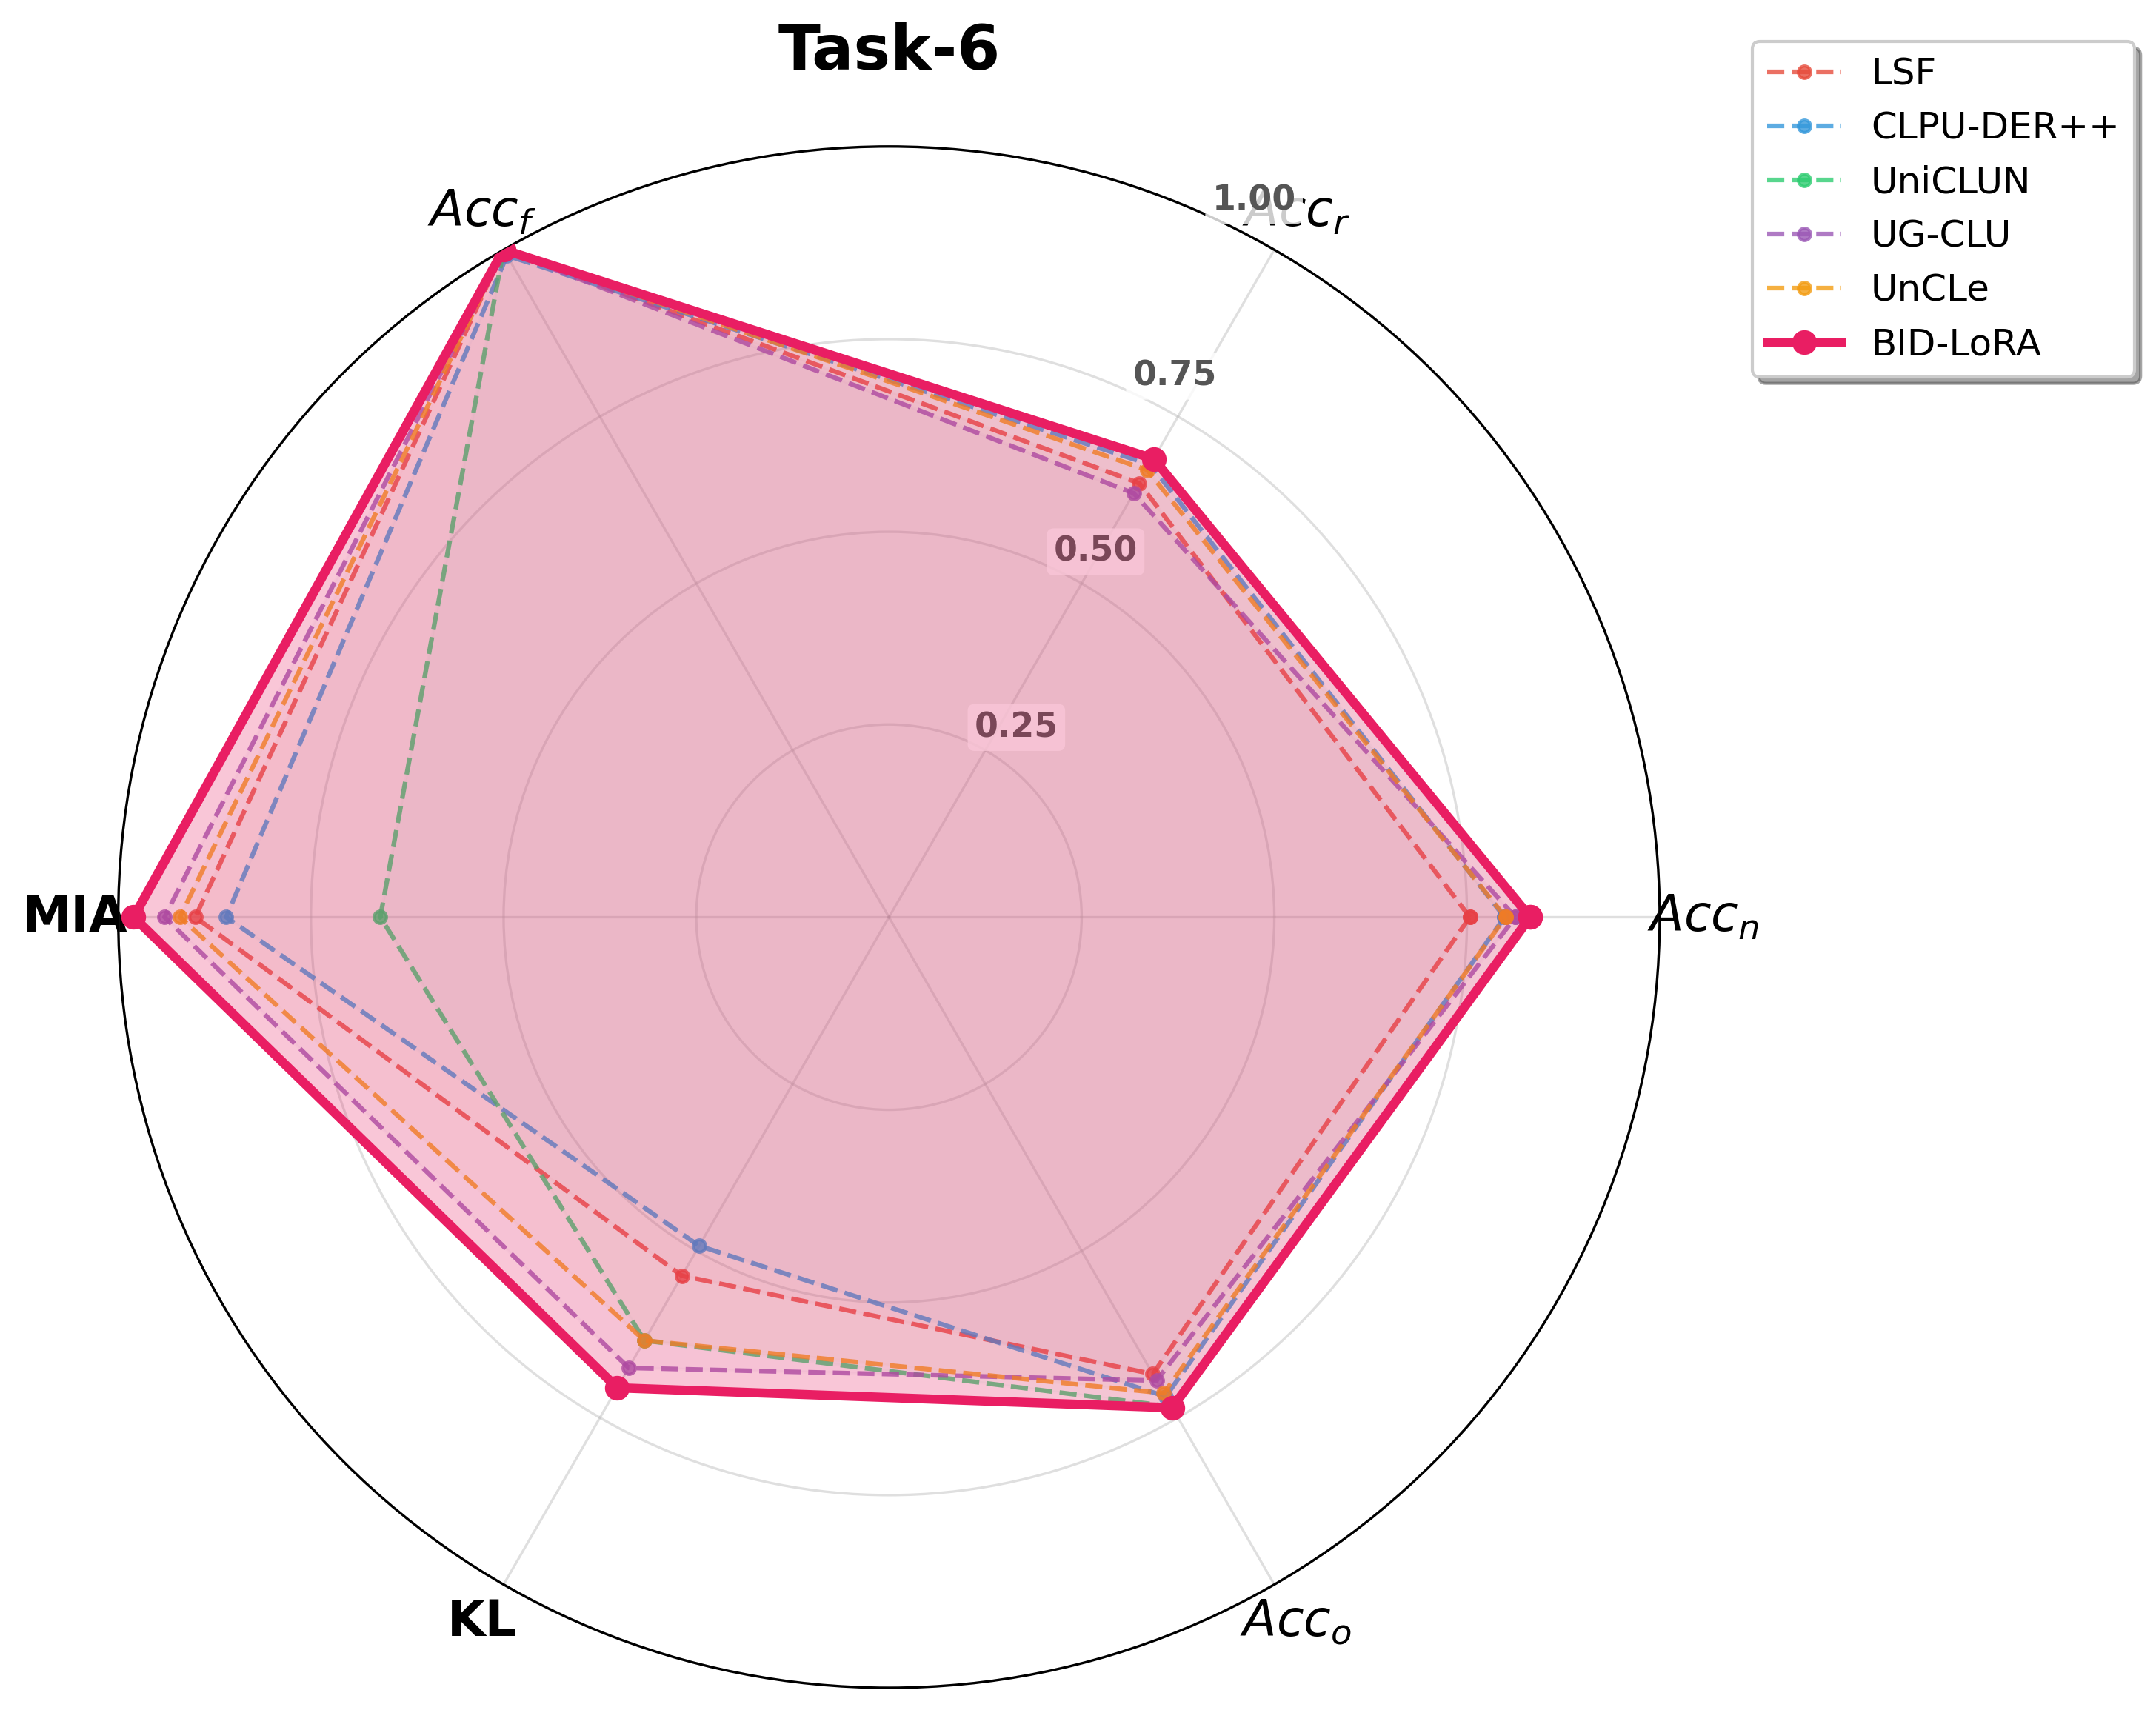
\includegraphics[width=\linewidth]{images/radar_task_6.png}
        \caption{Classification task}
    \end{subfigure}
    \hspace{0.5em}
    \begin{subfigure}[b]{0.38\linewidth}
        \centering
        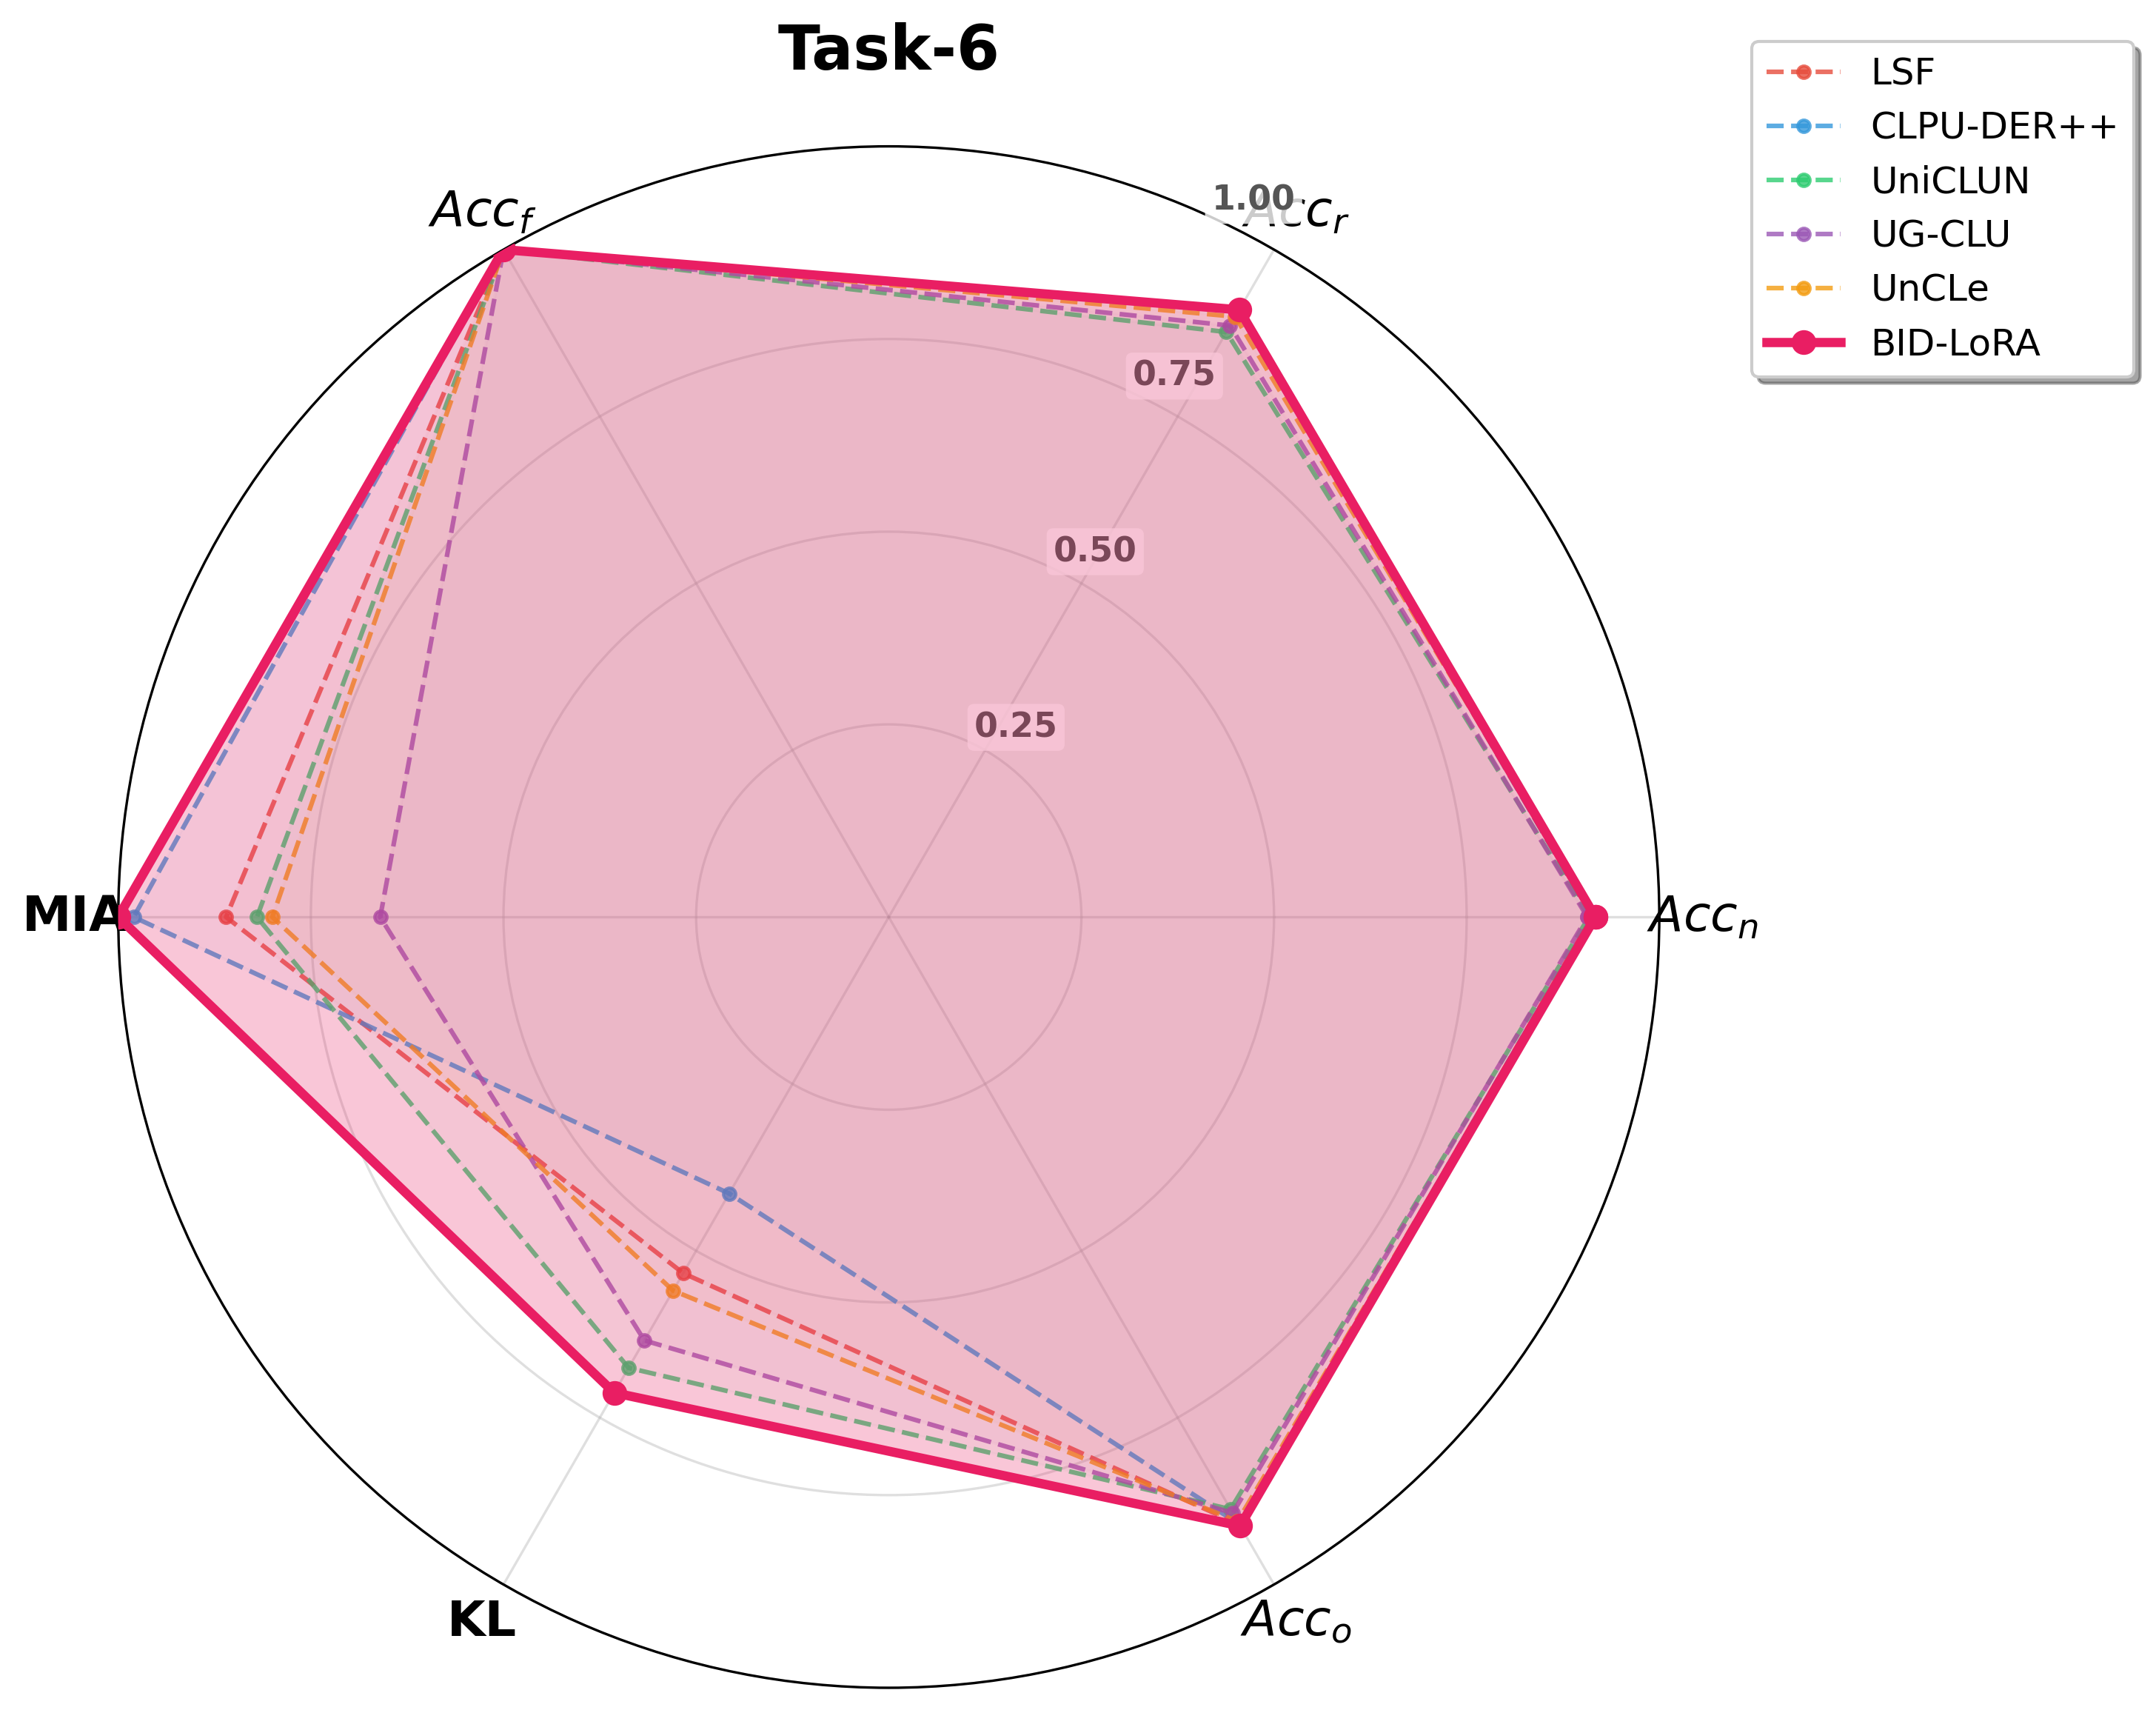
\includegraphics[width=\linewidth]{images/radar_task_6_face.png}
        \caption{Face recognition task}
    \end{subfigure}
    \caption{Radar plot comparison at Task-6. BID-LoRA consistently outperforms all baselines across metrics on both classification and face recognition tasks.}
    \label{fig:radar}
\end{figure}

\medskip
\noindent
\textit{Baseline Comparison:} Combined baseline methods exhibit conflicting optimization between their CL and MU components. LSF~\cite{shibata2021learning} achieves strong unlearning ($Acc_f = 0\%$ in most tasks) but sacrifices overall accuracy, dropping to 68.46\% in Task 6 on CIFAR-100. CLPU-DER++\cite{liu2022continual} and UniCLUN~\cite{chatterjee2024unified} demonstrate unstable retention accuracy, with UniCLUN's $Acc_r$ falling to 67.27\% by Task 2 on CIFAR-100. \textcolor{red}{MIA results for all baselines are reported in the ablation study (Section~\ref{7.0}).} \textcolor{red}{On face recognition, BID-LoRA achieves the best or second-best overall accuracy in 5 of 12 tasks, with $Acc_o$ of 89.69\%, 92.89\%, 92.29\%, 90.50\%, 87.97\%, 91.15\%, 87.03\%, 90.13\%, 89.16\%, 91.92\%, 91.70\%, and 92.61\% across Tasks 1--12 respectively.} As illustrated in Fig~\ref{fig:radar}, BID-LoRA's radar plot at Task-6 encloses all baseline methods, demonstrating superior performance across all evaluation metrics on both classification and face recognition tasks. Similar patterns are observed across CIFAR-100 and \textcolor{red}{VGGFace2} benchmarks.

\medskip
\noindent
\textit{Convergence Patterns:} BID-LoRA exhibits convergent behavior where new knowledge accuracy $Acc_n$ aligns closely with overall accuracy while retained accuracy $Acc_r$ remains stable. On CIFAR-100, new knowledge accuracy $Acc_n$ improves from \textcolor{red}{71.93\% in Task 1 to 80.20\%} in Task 6, while overall accuracy $Acc_o$ remains stable, moving from 76.03\% to 73.51\%, demonstrating effective knowledge acquisition without degrading cumulative performance. Retained accuracy maintains consistency across Tasks 2--6, ranging from \textcolor{red}{68.67\% to 72.33\%}, demonstrating that the bidirectional adapter architecture effectively balances learning and unlearning without catastrophic forgetting.